%! TEX root = ./master.tex

\lecture{07}{Week 4}{Wrapping up C}

\paragraph{C Preprocessor}
The C preprocessor (cpp) is not part of the language buts sits on top of it.

\paragraph{Include}
\code{\#include} is used to include header files inline in the source code. They provide a basic mechanism for for defining APIs.\\
Header files are either system header files, which are included using \code{<systemHeader>}, or own header files, included using \code{"ownHeader"}. We do not need to provide a path to the file, but the preprocessor will look at certain dedicated paths for the appropriate files.\\
It is important to \textbf{not} include a file twice. Also one should never include \code{.c} files.

\paragraph{Macros}
Macros provide token-based text substitution. A macro is defined using \code{\#define foo bar}. Any appearance of \code{foo} in the code is replaced with \code{baz}. Since macros are purely textual, we can use them for \textit{expressions} too. E.g. \code{\#define inc(x) (x + 1)} will replace \code{inc(1)} with \code{(1 + 1)}.\\
An undefined, or a defined macro which was removed using \code{\#undef foo} will evaluate to $1$ which evaluates to true in an expression.\\
Macros can span multiple lines and contains \textit{complex} structures by adding a backslash to the end of the line. The problem we may encounter with macros which represent a expression is that adding a semicolon after the term which gets replaced by the macro, results in two semicolons (if there is one in our macro too). When using the trick of \textit{Semicolon Swallowing}, we put our macro block inside a \code{do {ourMacro} while(0)} block. Adding a semicolon after the macro will no longer result in an error. The compiler removes the loop anyways.\\
An advantage of macros is to prevent overhead by inlining. But the compiler can do that by itself nowadays.

\paragraph{Conditionals}
Conditionals are useful to take different action at the build time. Preprocessors support conditionals of the form:
\begin{lstlisting}
\#if expression1
    (text1)
\#elif expression2
    (text2)
\#else
    (text3)
\#endif
\end{lstlisting}

Important is that expressions must be macros and literals only!

The conditional \code{\#ifdef foo} and \code{\#ifndef bar} evaluate to true or false depending whether the macro is defined or not. This is a shorthand for \code{\#if defined(foo)} and \code{\#if !defined(bar)}.

\subsubsection{Modularity}
A module is a self-contained piece of a larger program. It consists of an externally visible part, containing functions, typedefs, global variables, cpp macros (they define the module's interface) and of internal functions, types, variables which are hidden from the client.

\paragraph{Declaration vs Definition}
C differentiates between declaration and definition. A declaration is like the definition but without the body. Structs are declarations and cannot be defined.\\
A \textit{compilation unit} is a C source file and everything it includes. The compilation unit defines the visibility of definitions.\\
When we want to access a definition from another compilation unit (or the same) we prepend the declaration with \code{extern}. When prepending the declaration by \code{static}, this definition is only visible inside this compilation unit and cannot be accessed from the outside using \code{extern}.

\paragraph{Global Variables}
Global variables are also declared and the visibility can be controlled using \code{extern} as described above.

\paragraph{Header Files}
Header files specify interfaces and should not contain declarations (structs are definitions and not declarations). The module \code{foo} has the interface specified in \code{foo.h} and all clients of \code{foo} are required to include \code{\#include "foo.h"}. The implementation of \code{foo} is typically in the \code{foo.c}, which also must include \code{foo}. This source file ought not contain external declarations but only definitions and internal declarations.\\
The naming of \code{foo.c} and \code{foo.h} is just a convention which the compiler does not care about. For the execution simple the name of the definition matter.

\paragraph{CPP Convention}
One should never include the same header file twice or redeclare macros. Therefore, it is convenient to have a mechanism which prevents this. The following boilerplate ensures that:

\begin{lstlisting}
\#ifndef __FILE_H_
\#define __FILE_H_
(macros, headers)
\#endif
\end{lstlisting}

\code{\_\_FILE\_H\_} is the name if the program.

\subsubsection{Function Pointers}
Function pointers are pointers for functions. For example in \code{int (*funct)(int *, char);} \code{func} is a pointer to a function which takes two arguments, a pointer to int and a char. The return value of the function is int. Function pointers are rare in OOP languages, but they are sometimes referenced as \textit{delegates} or \textit{agents}.\\
Function pointers are very fundamental for a lot of techniques in system code. They allow for example to write \textit{object oriented like code} by having a struct of variables and functionpointers (sometimes called \textit{vtable}). This method does not provide any protection or hiding but does provide the benefit of reusability.

\subsubsection{Assertions}
Assertions evaluate an expression at runtime and crash the program if evaluated to false. In that case they print \code{"<filename>:<linenumber> <functionname>: Assertion <assertionexpression> failed."} and then abort.\\
Assertions are macros and using the compile flag \code{-DNDEBUG} they can be removed.

\subsubsection{goto}
Goto should be be used, except for:
\begin{itemize}
    \item Early termination of nested loops. But we may also put this in a dedicated function and return.
    \item Cleanup code. Like transactional memory, when one step fails, undo all previous steps. Depending on which stage failed, we need to undo a different number of steps.
\end{itemize}

The second usecase is visualized here:

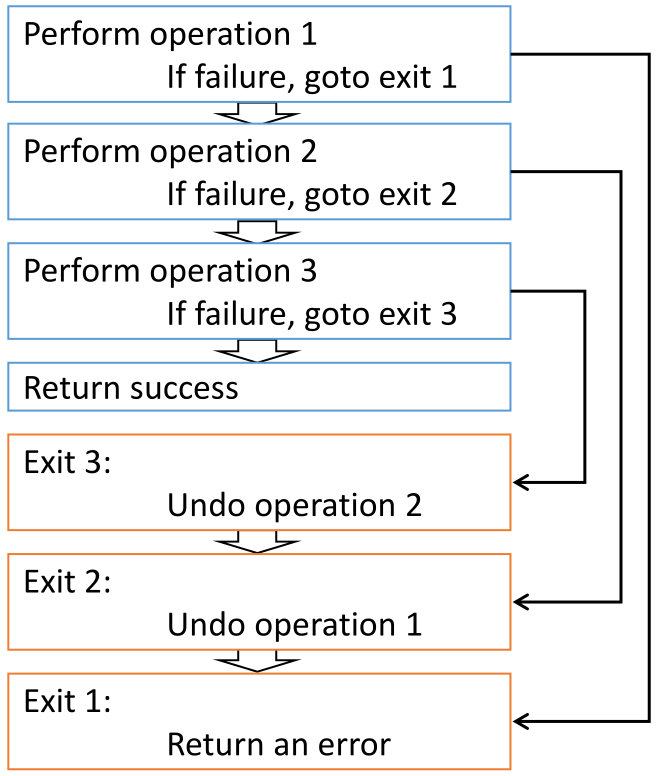
\includegraphics[width=0.8\textwidth]{07_CleanupCode.png}

\subsubsection{setjmp() and longjmp()}
The function \code{int setjmp\(jmp_buf env\)}, which must be imported with \code{<setjmp.h>}, saves the current stack state and environment to \code{env}. Then it returns $0$.

The function \code{void longjmp\(jmp_buf env, int val\)} takes a buffer of \code{setjmp} and causes the \code{setjmp} to return again the value of \code{val} or $1$ if $val = 0$. For each \code{setjmp}, this can only be done once and also only as long as the function containing \code{setjmp} has not returned.\\
This construct is very unique to C.

\subsubsection{Coroutine}
Coroutines are methods which are both at the top of the stack at the same times. Both routines should be able to call eachother to transfer e.g. data. They look similar to threads but they are not. In essence they allow dynamically switching between functions.

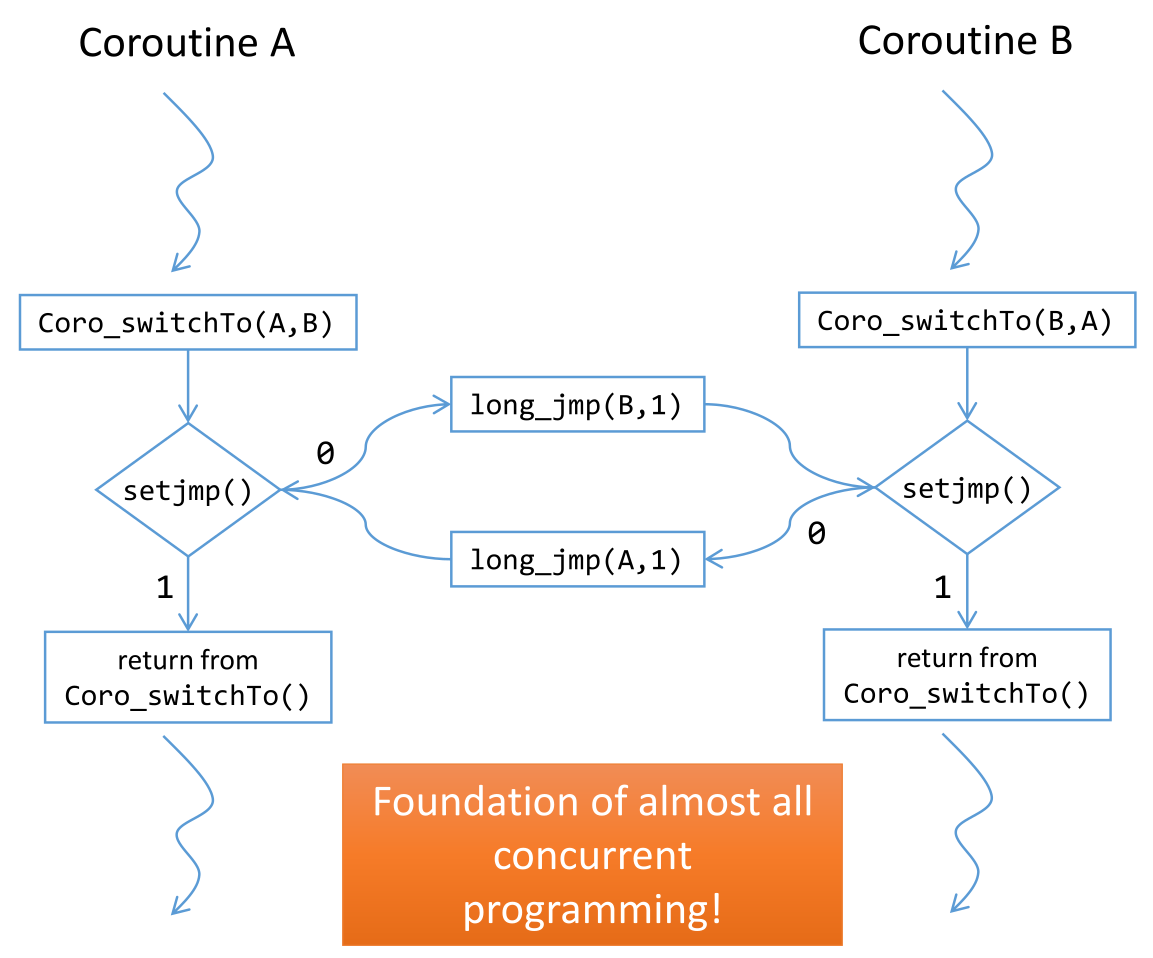
\includegraphics[width=0.8\textwidth]{07_coroutine.png}

Coroutines are completely based on \code{setjmp} and \code{longjmp}.

Coroutines are sometimes called \textit{Lightweight threads}, \textit{Protothreads}, \textit{Cooperative mtultitasking}... Thread based programming is based on this schema and we can make coroutines look like threads by dynamically switching into different functions. But there is no concurrently and no parallelism.

The comma is an operator which takes two statements. Both are evaluated, but only the second one is returned.
